% Public explainer for legibility-bounds, written for a non-specialist
% reader. Every number is taken from the committed records in results/,
% via the generated blocks in the README; the figures are the ones in
% docs/img/, produced by the repository's own tools.
%
% Build from this directory:  latexmk -pdf explainer.tex
%
% When the suite is re-run, the numbers in "The results", "What safety
% costs" and "Where the remaining width lives" must be re-checked against
% README.md, whose generated blocks come from results/. They are prose
% here, so nothing enforces them.
\documentclass[11pt,a4paper]{article}

\usepackage[margin=2.4cm,top=2.2cm,bottom=2.2cm]{geometry}
\usepackage[T1]{fontenc}
\usepackage[utf8]{inputenc}
\usepackage{lmodern}
\usepackage{microtype}
\usepackage{graphicx}
\usepackage{xcolor}
\usepackage{titlesec}
\usepackage{enumitem}
\usepackage{booktabs}
\usepackage[hidelinks]{hyperref}
\usepackage{fancyhdr}
\usepackage{tcolorbox}
\tcbuselibrary{skins,breakable}

\graphicspath{{../img/}}

\definecolor{navy}{HTML}{0F2F52}
\definecolor{gold}{HTML}{B08D3F}
\definecolor{ink}{HTML}{1A1A1A}
\definecolor{soft}{HTML}{F7F5F0}
\definecolor{rule}{HTML}{D8D3C8}

\color{ink}
\linespread{1.09}
\setlength{\parskip}{6pt}
\setlength{\parindent}{0pt}

\titleformat{\section}{\large\bfseries\color{navy}}{}{0pt}{}
\titlespacing*{\section}{0pt}{16pt}{6pt}

\pagestyle{fancy}
\fancyhf{}
\renewcommand{\headrulewidth}{0pt}
\fancyfoot[C]{\small\color{gray}\thepage}

\newtcolorbox{quotebox}[1][]{
  enhanced, breakable, colback=soft, colframe=gold,
  boxrule=0pt, leftrule=2.5pt, arc=0pt, outer arc=0pt,
  left=10pt, right=10pt, top=8pt, bottom=8pt, #1}

\newcommand{\code}[1]{{\ttfamily\small #1}}

\begin{document}

\begin{center}
{\LARGE\bfseries\color{navy} How good could it possibly be?}\\[6pt]
{\large Proving the limit of a robot's ability to make itself understood}\\[12pt]
{\small Munawar Kazmi \;\textbullet\; \href{https://munawarkazmi.com}{munawarkazmi.com}}\\[2pt]
{\small A plain-language guide to \textbf{legibility-bounds}, certified two-sided bounds on legible robot motion.}\\[2pt]
{\small Code, records, and every figure: \href{https://github.com/munawarkazmi/legibility-bounds}{github.com/munawarkazmi/legibility-bounds}}
\end{center}

\vspace{4pt}
{\color{rule}\hrule height 1pt}
\vspace{10pt}

\section{A robot walking towards one of three doors}

A robot sets off across a room. There are three doors it might be heading for, and from where you are standing, for the first few seconds, its movement is consistent with all three. You do not know whether to step aside, and which way.

A robot can fix this by moving deliberately: swinging wide early, in a way that only makes sense if it is going to the left-hand door. That is called \emph{legible} motion, and it costs something. The clearest route is longer than the shortest one, so a robot that wants to be understood has to spend distance to do it.

There is an established way of measuring how legible a given path is, and there are methods that try to find good ones. This project asks a question none of them can answer.

\section{The question nobody could answer}

Suppose you design a test room, run the best available method in it, and it produces a trajectory scoring 0.58 out of 1.

Is that good?

You genuinely cannot tell. Two completely different explanations fit:

\begin{itemize}[leftmargin=1.4em,itemsep=2pt]
\item The room is simply hard. Perhaps the doors are positioned so that no route can signal your intention early, and 0.58 is close to the best anything could do.
\item Or the room is fine and your method underperformed, and something better exists that nobody has found yet.
\end{itemize}

Every existing approach searches for good trajectories and reports the best it found. A search can only ever tell you \textbf{something at least this good exists}. It can never tell you that nothing better does, because the thing it did not find might be just outside where it looked.

\begin{quotebox}
So the question a scenario designer actually asks, \emph{is this world hard, or did my planner just do badly in it?}, has had no answer. You cannot tell a difficult room from a disappointing algorithm.
\end{quotebox}

\section{The other kind of claim}

This project supplies the missing half. For a given room, a given budget on extra distance, and a stated model of the watching person, it returns two numbers:

\begin{itemize}[leftmargin=1.4em,itemsep=2pt]
\item a trajectory that \textbf{does} achieve a certain legibility, which you can inspect, and
\item a level that \textbf{no} trajectory within the budget can reach, ever.
\end{itemize}

The true best possible value lies between them, and the distance between them is published rather than hidden.

That second number is a different kind of statement from anything a search produces. It is negative, and it covers \emph{every} route the robot could take rather than the handful that were tried. No amount of further computation overturns it, and a cleverer optimiser arriving next year does not weaken it.

Here is a real one, from the committed results:

\begin{quotebox}
\textit{No trajectory from the start to the true goal in the} \code{wall\_choice} \textit{room, spending at most 50 per cent more distance than the shortest route, attains a legibility of \textbf{0.81 or above} under this observer.}\\[4pt]
\textit{One attaining \textbf{0.8004} exists.}
\end{quotebox}

The shortest route in that room scores 0.5457, so the extra distance genuinely buys clarity. And the two ends sit 0.0064 apart, which means any target outside that narrow band is now settled: above it, provably unreachable; at or below the achieved value, definitely reached.

\section{How you prove something about every possible route}

Proving that \emph{no} path can do better sounds impossible, since there are infinitely many paths. It becomes possible because of two facts about the measurement that are not obvious from its definition.

\textbf{First, the watcher's belief depends only on where the robot is, not how it got there.} Working through the arithmetic of the observer's reasoning, the distance already travelled cancels out entirely. So the belief across the whole room can be computed once, as a fixed map, before considering any trajectory at all. That is the shaded field in the figure below: dark where a robot standing there would have convinced you it is going to goal A.

\textbf{Second, the measurement does not care how long the journey takes.} The weighting that emphasises early clarity divides by its own total, so overall duration cancels too. The bound never has to consider how fast the robot moves.

\begin{figure}[t]
\centering
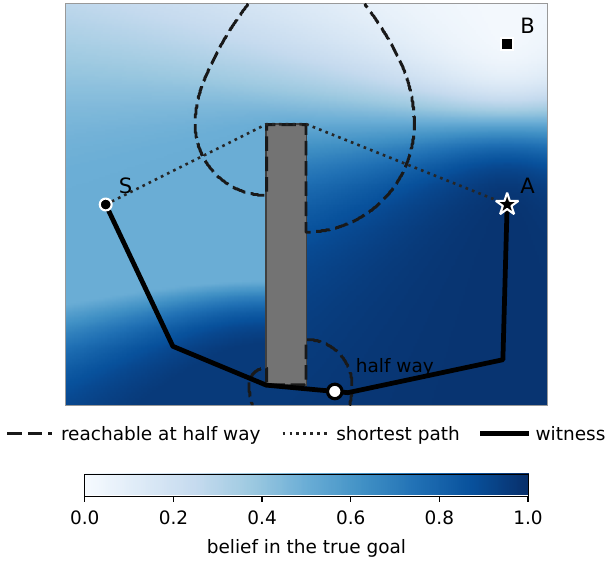
\includegraphics[width=0.72\linewidth]{mechanism.png}
\caption{\small One room. Shading is how strongly a watcher would believe in goal A if the robot were standing at that point. The dashed shape is everywhere the robot could possibly be at the halfway point of its journey, given its distance budget. The dotted line is the shortest route; the solid line is the constructed trajectory that achieves the lower end of the certified interval.}
\end{figure}

The proof then comes from simple geography. Consider the robot halfway through its journey. If its total path is limited, it cannot be further from the start than the distance it has had time to cover, and it cannot be further from the goal than the distance it has left. Those two limits carve out a lens-shaped region, drawn dashed above, and the robot is definitely somewhere inside it.

So: find the highest belief value anywhere in that lens. The robot's actual belief at the halfway point cannot exceed it, whatever route it took. Do that for every point along the journey, add up the results, and you have an upper limit that holds for every admissible trajectory simultaneously.

\section{The wall problem, and the way around it}

That argument works cleanly in an empty room. Obstacles break it.

The reason is that in a room with walls, closeness is not what it appears. Two points a centimetre apart on opposite sides of a wall are, to a robot that must walk around, separated by the entire length of the wall. The usual way of arguing that belief cannot change much across a small region relies on nearby points behaving similarly, and beside a wall they do not.

The fix is a change of bookkeeping. Instead of tracking belief directly, the argument tracks the \emph{odds against} the true goal. Bounding that from above turns out to need only a lower limit on the \emph{difference} between two walking distances, rather than a limit on each one separately. And that difference stays well-behaved precisely where the individual distances do not.

It is a small reformulation that rescues the whole argument next to obstacles, and it is the step the work turns on.

\section{Building the other end rather than searching for it}

The upper limit is only half an interval. The lower end needs an actual trajectory.

The obvious approach is to run a search. This project deliberately does not, because a search is exactly the thing it exists not to rely on. Instead the trajectory is \emph{constructed}: it is threaded through the high-belief cells that the bound itself identified, joined up with exact shortest connections, and then pulled back towards the direct route until it fits inside the distance budget. It is then scored by the same measurement as everything else, so what it claims is what it measures.

This turns out to work better than searching, too. Against the reference local search, the constructed trajectory is the better of the two in \textbf{13 of 32} cases, by as much as 0.1485. Where the search wins, the search's number is used and the record says which produced it.

\section{The results}

\begin{figure}[t]
\centering
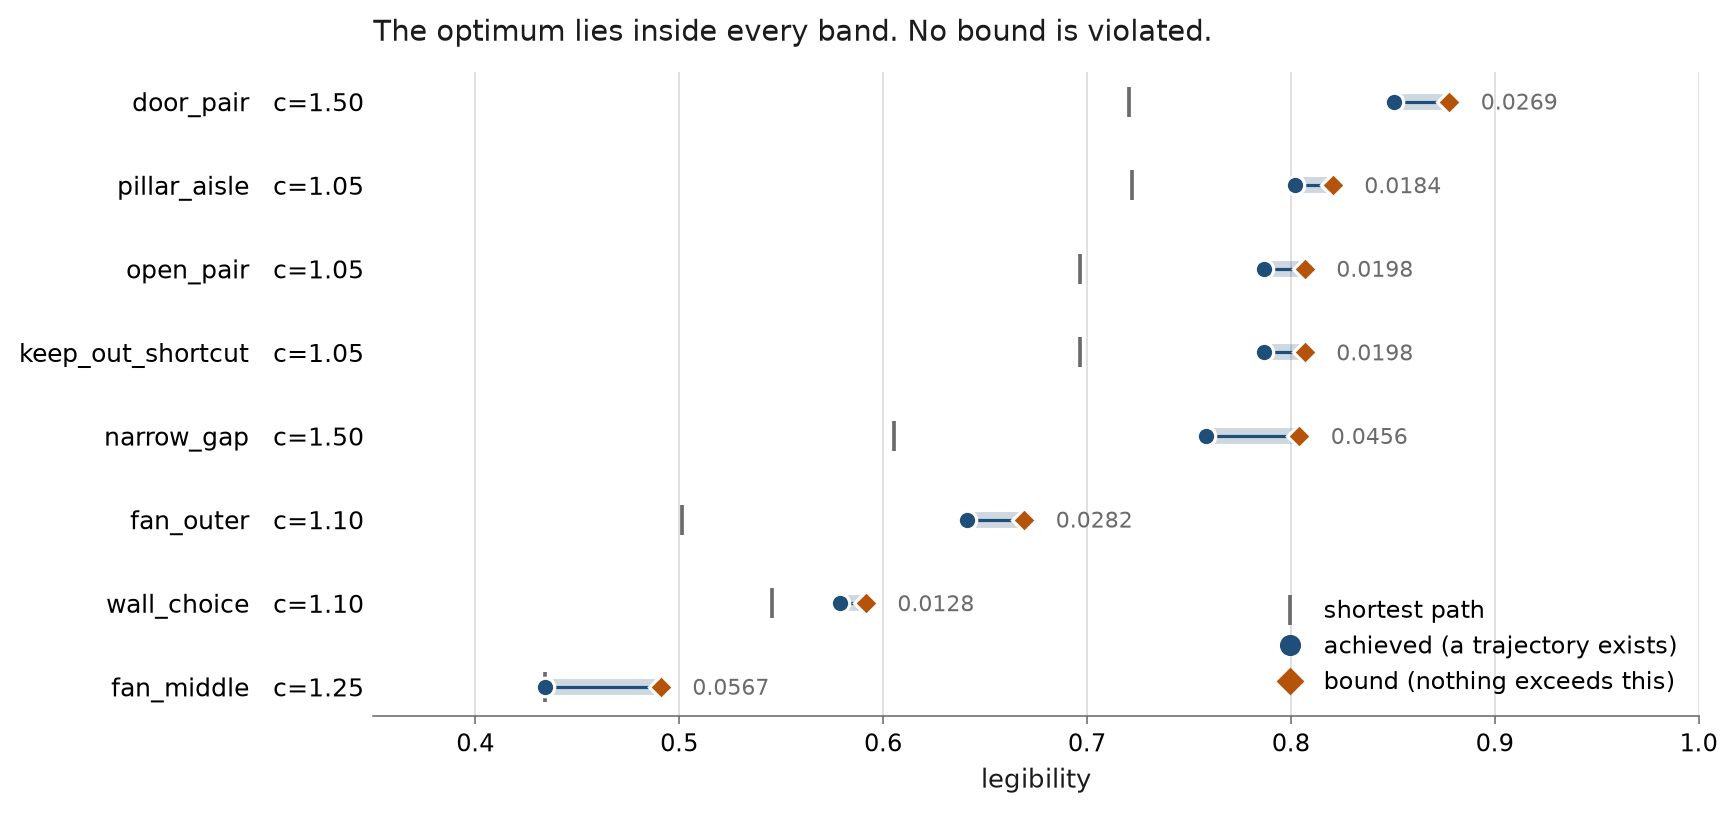
\includegraphics[width=\linewidth]{intervals.png}
\caption{\small Every band is a certified interval. The circle is a trajectory that exists, the diamond is a level nothing can exceed, and the tick marks the shortest route for contrast. The best possible value lies inside every band.}
\end{figure}

Eight rooms, four distance budgets each, so 32 combinations in total. \textbf{Every one holds, with no violations.} The intervals range from 0.0064 apart at the tightest to 0.0567 at the widest.

Look at how far the circles sit from the ticks: in most rooms, spending a little extra distance buys a great deal of clarity. And look at how far apart the rooms are from one another. That spread is the thing that was previously invisible. Some of these rooms are simply harder than others, and now that can be stated rather than suspected.

\section{What safety costs, provably}

There is a second result, and it is arguably the more useful one.

Suppose the room has a region the robot should stay out of. How much clarity does respecting it cost? The natural approach is to run your method twice, with and without the restriction, and compare.

That comparison establishes nothing. If the restricted run scores worse, it may be because the restriction genuinely costs something, or it may be because that particular search happened to do worse. You cannot separate the two.

The bound settles it, because a keep-out region restricts the robot but not the person watching, so the same argument applies to the restricted problem. Put that limit next to an unrestricted trajectory that demonstrably exists, and if the achievable value is higher than the restricted ceiling, the gap between them is a \textbf{certified minimum price} of the safety constraint. Something is achievable; nothing safe can match it.

\begin{center}
\small
\begin{tabular}{lrrrr}
\toprule
room & budget & achievable & safe ceiling & certified price \\
\midrule
\code{pillar\_aisle} & 1.05 & 0.8022 & 0.7558 & \textbf{0.0464} \\
\code{keep\_out\_shortcut} & 1.25 & 0.8353 & 0.8225 & \textbf{0.0128} \\
\code{keep\_out\_shortcut} & 1.10 & 0.8079 & 0.8009 & \textbf{0.0070} \\
\bottomrule
\end{tabular}
\end{center}

Three of the eight cases certify a positive price. The other five certify nothing, and are reported as nothing rather than as zero.

One detail is worth drawing out. In \code{keep\_out\_shortcut} the cheapest route is already safe, so the restriction costs a robot nothing at all, as long as that robot is not trying to be understood. The price only appears once the robot wants to communicate. Being both safe and clear is harder than being either.

\section{Where the remaining width lives}

The intervals are not tight, and rather than leave that as a caveat, the project measures where the slack actually is.

One suspected cause was ruled out by testing rather than argument: a deliberately discarded piece of the reasoning turns out to be worth less than a hundredth of a point, and recovering it would cost more than the alternative.

Most of the remaining width comes from the resolution of the grid the room is divided into. Refining that grid closes between 55 and 79 per cent of the gap, which means the published numbers are conservative by roughly that margin.

What survives even that is a single constant in the obstacle argument. The proof guarantees a detour of no more than about 6.14 cell-widths near a corner; measuring actual points beside actual corners, each to its own grid point, finds the worst real detour is 0.99. So the constant is loose by a factor of about 6.2.

\begin{quotebox}
That is not an error, because a proof must hold in the worst case and the worst case is rarely met. What it is not is the prize this section used to call it.
\end{quotebox}

An earlier version of this page said something stronger and less true, so it is worth setting out what changed. The constant used to be about 9.28, and a sharper argument brought it to 6.14. That was expected to matter and it did not. It closed 1.6 per cent of the total width, because most of the rooms draw nothing from the obstacle argument at all and cannot move however tight it becomes. Refining the grid, at 55 to 79 per cent, is worth some forty times as much.

The looseness was also being measured in a way that flattered the constant. It compared two arbitrary points of a cell, which is a harder distance than the proof ever claims, and it drew those points from a box wider than the cell itself. Measured correctly, no sampled point in any room tested is cut off from its own grid point at all, and the detour argument never actually binds.

\section{How much of that gap could anyone close?}

The figure of 6.2 answers a narrower question than it appears to. It says how much slack there is in \emph{these} rooms. It says nothing about how much of that slack a better proof could ever take back, and those are different questions with different answers.

Answering the second one means putting the measuring tape away and building a room on purpose. Place a single obstacle beside a grid point, arranged as awkwardly as the rules still allow, and ask how far a nearby point genuinely is from that grid point once you are forced to walk around the obstacle rather than through it. The answer is 3.49 cell-widths. That room is legal, so no proof is allowed to promise anything smaller than 3.49, however clever it is.

\begin{quotebox}
So the gap splits in two. A sharper argument could bring the guarantee from 6.14 down to about 3.49, a factor of 1.76, and there it stops. The rest is not slack in the proof at all.
\end{quotebox}

What is left over is the distance between the rooms in this suite and the nastiest room the rules permit. No amount of cleverness recovers it, because there is nothing there to recover: the proof has to survive the nasty room, and these rooms simply are not it. That is worth separating out, because "the guarantee is six times larger than anything we measured" sounds like six times of waiting improvement, and only a fraction of it is.

The obstacle in that awkward room is narrower than a single cell. That sounds like cheating and is the opposite. An earlier version of the rules required every obstacle to be wider than a cell, and that requirement was withdrawn, because width is a property of a whole shape and a long thin triangle can be broad overall while its tip is thinner than a cell and slips straight through one. The rule in force is checked cell by cell instead. The awkward room obeys the rule that is actually in force, which is exactly why it constrains the constant actually in use.

One thing this does not settle. 3.49 is the worst room anyone has built, not a proof that no worse room exists. The true answer lies somewhere between 3.49 and 6.14, and finding it is an open question rather than a finished one.

Publishing the location of your own weakest step, with a measurement of how weak it is, is unusual. Publishing that the step you named as weakest was not the one that mattered, that you had been measuring it against the wrong quantity, and that most of what remains was never available to begin with, is the same discipline turned on itself. It is the reason the rest of the numbers can be taken at face value.

\section{What is not true}

The repository has a section with this heading, and it is not decoration.

\textbf{The watching observer is a model, not a person.} It is precisely defined and exactly reproducible, and it has never been tested against what a human watching the robot would actually conclude. Everything here is a certified bound on a stated mathematical objective. Whether that objective matches human perception is a separate question, and an open one.

\textbf{The observer cannot be confused.} Its beliefs always sum to one across the declared goals, no matter how strange the robot's motion becomes. It can never think ``neither of those''. This is a known direction of error and it grows as the robot spends more distance.

\textbf{One definition, among several.} Legibility is not a single agreed quantity in this field. What is bounded here is one specific formulation, and a bound on it says nothing about the others.

\textbf{Obstacles must be convex shapes}, with a condition checked for each grid cell; cells failing it fall back to a weaker bound that always holds. And everything rests on one grid resolution, one observer setting, and one search budget. Nothing here is a trend.

\section{Why it matters}

Robots that share space with people need to be readable, and there is now a growing body of work on making them so. All of it, until now, has been able to say only that something reasonably good was found.

Being able to say what is \emph{impossible} changes what the field can do. A scenario can be certified as genuinely difficult rather than merely unsolved. A method can be judged against the true ceiling instead of against whatever the previous method managed. And the cost of a safety rule can be established as a fact about the problem, rather than as the difference between two runs that might both have been unlucky.

\vspace{6pt}
{\color{rule}\hrule height 1pt}
\vspace{6pt}

{\small Every bound, every trajectory, every figure and the code that produces them are public. No number in the repository's front page is typed by hand: all of it is regenerated from committed records, with a check that fails if it goes stale. The geometry comes from a companion project, pinned to an exact version so a bound cannot drift from the benchmark it bounds.\\
Repository: \href{https://github.com/munawarkazmi/legibility-bounds}{github.com/munawarkazmi/legibility-bounds}}

\end{document}
